%%%%%%%%%%%%%%%%%%%%%%%%%%%%%%%%%%%%%%%%%%%%%%%%%%%%%%%%%%%%%%%%%%
%%	    mmm  mmmmmm mm   m        m    m mmmmmm mmmmmm          %%
%%	  m"   " #      #"m  #        #    # #           #      	%%
%%	  #   mm #mmmmm # #m #        #    # #mmmmm     #        	%%
%%	  #    # #      #  # #  """   #    # #         #	        %%
%%	   "mmm" #mmmmm #   ##        "mmmm" #mmmmm  #          	%%
%%								                                %%
%%                                                              %%
%%                                                              %%
%%      Grundlagen der Elektrischen Netzwerke, UE               %%
%%      Gruppe 5, Team F                                        %%
%%      Authors: Severin Wolf, Maximilian Seidler.              %%
%%%%%%%%%%%%%%%%%%%%%%%%%%%%%%%%%%%%%%%%%%%%%%%%%%%%%%%%%%%%%%%%%%
\documentclass[a4paper]{article}

\usepackage{pstricks}
\usepackage{pst-circ}
\usepackage{pst-plot}
\usepackage{pstricks-add}
\usepackage{amsmath}
\usepackage[utf8]{inputenc}
\usepackage[ngerman, english]{babel} 
\usepackage{geometry}
\geometry{a4paper,left=3cm,right=2cm, top=2cm, bottom=2cm} 
\usepackage{graphicx}
\usepackage[EFvoltages, european, straightvoltages]{circuitikz}

\newpsobject{showgrid}{psgrid}{subgriddiv=1,griddots=10,gridlabels=0pt}
\psset{unit=1.0cm}
\psset{tensioncolor=blue}
\psset{tensionlabelcolor=blue}
\psset{intensitycolor=red}
\psset{intensitylabelcolor=red}

\setlength{\parindent}{0pt}
\usepackage{lipsum}

\newcommand\blfootnote[1]{%
	\begingroup
	\renewcommand\thefootnote{}\footnote{#1}%
	\addtocounter{footnote}{-1}%
	\endgroup
}

\begin{document}
\pagestyle{empty} \enlargethispage*{25cm}\samepage{

\vspace*{-3cm}
\begin{center}
\begin{minipage}[!h]{18cm}
\hspace*{-0.9cm}
\includegraphics[width=3.3cm]{./Figures/igte_logo}
\begin{tabular}{p{10cm}}
\vspace{0.5cm}
\centering{
	\Large Institute of Fundamentals and Theory in
	Electrical Engineering\\
	Graz University of Technology\\
	~\\}
\end{tabular}
\includegraphics[width=3.3cm]{./Figures/TUG_logo}
\end{minipage}
	\Large
	\textbf{Fundamentals of Electrical Circuits} \vspace*{0.5cm}\\
	\textbf{Homework 7}\\
	Laplace-Transformation
	\vspace*{0.5cm}
	
	\large
	6 May 2021
	\end{center}}

	\vspace*{1cm}
	
	%%%%%%%%%%%%%%%%%%%%%%%%%%%%%%%%%%%%%%%%%%%%%%%%%%%%%%%%%%%%%%%%%%%%
	%%%%%%%%%%%%%%%%%%%%%%%%%%%%%%%%%%%%%%%%%%%%%%%%%%%%%%%%%%%%%%%%%%%%
	Apply the Laplace-Transform in order to analyse the given circuit.
	\begin{enumerate}
		\item Apply the Laplace-Transform in oder to compute $U(s) = \mathcal{L}\{u(t)\}$ in the s-domain. \\
		$u(t)$ is defined by the diagram in figure \ref{fig:input}. \textbf{(0.5 Points)}
		
		\item Derive the s-domain equivalent circuit and include the possibility of inital values. \textbf{Mark the current through the capacitor in the s-domain cirucit.} Pay attention to the arrow's direction. \textbf{(0.5 Points)}
		
		\item Derive the expression for the voltage across the capacitor $U_C(s)$ in the s-domain by applying KCL and KVL to the circuit. The initial condition for the capacitor is given as $u_C(t=0) = 0\,\text{V}$ and can be used to simplify the equations. \textbf{(1 Point)}

		\item Find the time-domain expressions for the voltage $u_C(t) = \mathcal{L}^{-1}\{U_C(s)\}$ for the given input signal. Calculate the time constant $\tau$ for this first order circuit. \textbf{(1.5 Points)}

		\item Plot the voltage $u_C(t)$ across the capacitor for $0 \leq t \leq 4T$ in \textsc{Matlab}. \textbf{(0.5 Points)}
		
		\item Simulate the circuit in LTSpice for the given input voltage $u(t)$ for the same time-intervall and compare the results. \textbf{(1 Point)}
	\end{enumerate}
		

	\subsection*{Values:}
	$R_1 = 100~\Omega$ \qquad $R_2 = 100~\Omega$ \qquad $R_3 = 300~\Omega$ \qquad $C=25~\mu\text{F}$ \qquad $U_0 = 2.5~\text{V}$ \qquad $T = 4~\text{ms}$\\
	
	\begin{figure}[!htb]
		\begin{minipage}{0.4\textwidth}
			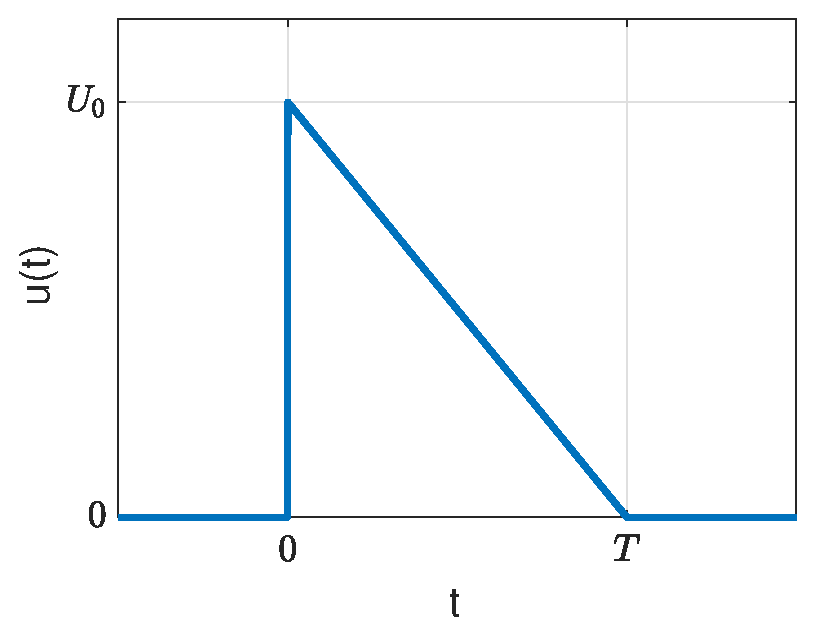
\includegraphics[width=1\textwidth]{./Figures/input-signal.eps}
			\caption{Input-Signal}
			\label{fig:input}
		\end{minipage}\hfill
		\begin{minipage}{0.4\textwidth}
			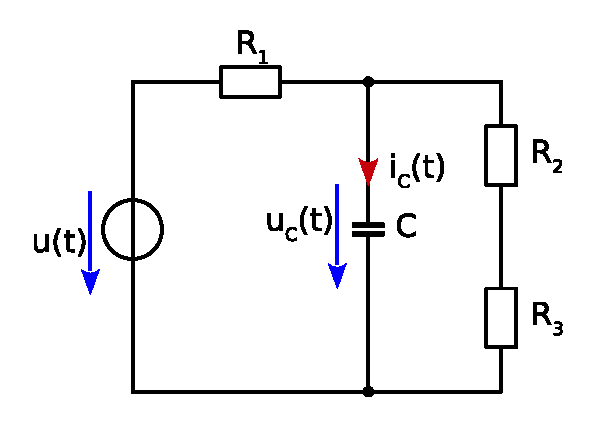
\includegraphics[width=1\textwidth]{./Figures/homework7_circuit.eps}
			\caption{Circuit}
			\label{fig:circuit}
			\vspace{1cm}
		\end{minipage}
	\end{figure}
	
	
	\blfootnote{Deadline: 13 May 2021; Presentation: Team 7 \\
		presentation: 14 May 2021 at 9o'Clock (attendence is voluntary!) \\
	Link to the presentation-meeting: https://tugraz.webex.com/tugraz/j.php?MTID=ma0812eff6637ffbf004e8bab03ee5f70}

\end{document}